\documentclass[dutch]{mimosis}
\usepackage{metalogo}
\usepackage{tabularx}

%%%%%%%%%%%%%%%%%%%%%%%%%%%%%%%%%%%%%%%%%%%%%%%%%%%%%%%%%%%%%%%%%%%%%%%%
% Some of my favourite personal adjustments
%%%%%%%%%%%%%%%%%%%%%%%%%%%%%%%%%%%%%%%%%%%%%%%%%%%%%%%%%%%%%%%%%%%%%%%%
%
% These are the adjustments that I consider necessary for typesetting
% a nice thesis. However, they are *not* included in the template, as
% I do not want to force you to use them.

% This ensures that I am able to typeset bold font in table while still aligning the numbers
% correctly.
\usepackage{etoolbox}

\usepackage[binary-units=true]{siunitx}
\DeclareSIUnit\px{px}

\sisetup{%
  detect-all           = true,
  detect-family        = true,
  detect-mode          = true,
  detect-shape         = true,
  detect-weight        = true,
  detect-inline-weight = math,
}

%%%%%%%%%%%%%%%%%%%%%%%%%%%%%%%%%%%%%%%%%%%%%%%%%%%%%%%%%%%%%%%%%%%%%%%%
% Hyperlinks & bookmarks
%%%%%%%%%%%%%%%%%%%%%%%%%%%%%%%%%%%%%%%%%%%%%%%%%%%%%%%%%%%%%%%%%%%%%%%%

\usepackage[%
  colorlinks = true,
  citecolor  = RoyalBlue,
  linkcolor  = RoyalBlue,
  urlcolor   = RoyalBlue,
  ]{hyperref}

\usepackage{bookmark}
\usepackage[shortlabels]{enumitem}
\usepackage{float}

%%%%%%%%%%%%%%%%%%%%%%%%%%%%%%%%%%%%%%%%%%%%%%%%%%%%%%%%%%%%%%%%%%%%%%%%
% Bibliography
%%%%%%%%%%%%%%%%%%%%%%%%%%%%%%%%%%%%%%%%%%%%%%%%%%%%%%%%%%%%%%%%%%%%%%%%
%
% I like the bibliography to be extremely plain, showing only a numeric
% identifier and citing everything in simple brackets. The first names,
% if present, will be initialized. DOIs and URLs will be preserved.

\usepackage[%
  autocite     = plain,
  backend      = bibtex,
  doi          = true,
  url          = true,
  giveninits   = true,
  hyperref     = true,
  maxbibnames  = 99,
  maxcitenames = 99,
  sortcites    = true,
  style        = numeric,
  ]{biblatex}

%%%%%%%%%%%%%%%%%%%%%%%%%%%%%%%%%%%%%%%%%%%%%%%%%%%%%%%%%%%%%%%%%%%%%%%%
% Some adjustments to make the bibliography more clean
%%%%%%%%%%%%%%%%%%%%%%%%%%%%%%%%%%%%%%%%%%%%%%%%%%%%%%%%%%%%%%%%%%%%%%%%
%
% The subsequent commands do the following:
%  - Removing the month field from the bibliography
%  - Fixing the Oxford commma
%  - Suppress the "in" for journal articles
%  - Remove the parentheses of the year in an article
%  - Delimit volume and issue of an article by a colon ":" instead of
%    a dot ""
%  - Use commas to separate the location of publishers from their name
%  - Remove the abbreviation for technical reports
%  - Display the label of bibliographic entries without brackets in the
%    bibliography
%  - Ensure that DOIs are followed by a non-breakable space
%  - Use hair spaces between initials of authors
%  - Make the font size of citations smaller
%  - Fixing ordinal numbers (1st, 2nd, 3rd, and so) on by using
%    superscripts

% Remove the month field from the bibliography. It does not serve a good
% purpose, I guess. And often, it cannot be used because the journals
% have some crazy issue policies.
% \AtEveryBibitem{\clearfield{month}}
% \AtEveryCitekey{\clearfield{month}}

% Fixing the Oxford comma. Not sure whether this is the proper solution.
% More information is available under [1] and [2].
%
% [1] http://tex.stackexchange.com/questions/97712/biblatex-apa-style-is-missing-a-comma-in-the-references-why
% [2] http://tex.stackexchange.com/questions/44048/use-et-al-in-biblatex-custom-style
%
\AtBeginBibliography{%
  \renewcommand*{\finalnamedelim}{%
    \ifthenelse{\value{listcount} > 2}{%
      \addcomma
      \addspace
      \bibstring{and}%
    }{%
      \addspace
      \bibstring{and}%
    }
  }
}

% Suppress "in" for journal articles. This is unnecessary in my opinion
% because the journal title is typeset in italics anyway.
\renewbibmacro{in:}{%
  \ifentrytype{article}
  {%
  }%
  % else
  {%
    \printtext{\bibstring{in}\intitlepunct}%
  }%
}

% Remove the parentheses for the year in an article. This removes a lot
% of undesired parentheses in the bibliography, thereby improving the
% readability. Moreover, it makes the look of the bibliography more
% consistent.
\renewbibmacro*{issue+date}{%
  \setunit{\addcomma\space}
    \iffieldundef{issue}
      {\usebibmacro{date}}
      {\printfield{issue}%
      \setunit*{\addspace}%
      \usebibmacro{date}}%
  \newunit}

% Delimit the volume and the number of an article by a colon instead of
% by a dot, which I consider to be more readable.
\renewbibmacro*{volume+number+eid}{%
  \printfield{volume}%
  \setunit*{\addcolon}%
  \printfield{number}%
  \setunit{\addcomma\space}%
  \printfield{eid}%
}

% Do not use a colon for the publisher location. Instead, connect
% publisher, location, and date via commas.
\renewbibmacro*{publisher+location+date}{%
  \printlist{publisher}%
  \setunit*{\addcomma\space}%
  \printlist{location}%
  \setunit*{\addcomma\space}%
  \usebibmacro{date}%
  \newunit%
}

% Ditto for other entry types.
\renewbibmacro*{organization+location+date}{%
  \printlist{location}%
  \setunit*{\addcomma\space}%
  \printlist{organization}%
  \setunit*{\addcomma\space}%
  \usebibmacro{date}%
  \newunit%
}

% Display the label of a bibliographic entry in bare style, without any
% brackets. I like this more than the default.
%
% Note that this is *really* the proper and official way of doing this.
\DeclareFieldFormat{labelnumberwidth}{#1\adddot}

% Ensure that DOIs are followed by a non-breakable space.
\DeclareFieldFormat{doi}{%
  \mkbibacro{DOI}\addcolon\addnbspace
    \ifhyperref
      {\href{http://dx.doi.org/#1}{\nolinkurl{#1}}}
      %
      {\nolinkurl{#1}}
}

% Use proper hair spaces between initials as suggested by Bringhurst and
% others.
\renewcommand*\bibinitdelim {\addnbthinspace}
\renewcommand*\bibnamedelima{\addnbthinspace}
\renewcommand*\bibnamedelimb{\addnbthinspace}
\renewcommand*\bibnamedelimi{\addnbthinspace}

% Make the font size of citations smaller. Depending on your selected
% font, you might not need this.
\renewcommand*{\citesetup}{%
  \biburlsetup
  \small
}

\DeclareLanguageMapping{english}{english-mimosis}

\addbibresource{bibliography.bib}

%%%%%%%%%%%%%%%%%%%%%%%%%%%%%%%%%%%%%%%%%%%%%%%%%%%%%%%%%%%%%%%%%%%%%%%%
% Fonts
%%%%%%%%%%%%%%%%%%%%%%%%%%%%%%%%%%%%%%%%%%%%%%%%%%%%%%%%%%%%%%%%%%%%%%%%

\ifxetexorluatex
  \setmainfont{Minion Pro}
\else
  \usepackage[lf]{ebgaramond}
  \usepackage[oldstyle,scale=0.7]{sourcecodepro}
  \singlespacing
\fi

\renewcommand{\th}{\textsuperscript{\textup{th}}\xspace}

\newacronym[description={Artificiële Intelligentie}]{AI}{AI}{artificiële intelligentie}


\newacronym[description={Text-to-speech}]{TTS}{TTS}{text-to-speech}
   


\newglossaryentry{LaTeX}{%
  name        = {\LaTeX},
  description = {A document preparation system},
  sort        = {LaTeX},
}

\newglossaryentry{Real numbers}{%
  name        = {$\real$},
  description = {The set of real numbers},
  sort        = {Real numbers},
}

\makeindex
\makeglossaries

%%%%%%%%%%%%%%%%%%%%%%%%%%%%%%%%%%%%%%%%%%%%%%%%%%%%%%%%%%%%%%%%%%%%%%%%
% Incipit
%%%%%%%%%%%%%%%%%%%%%%%%%%%%%%%%%%%%%%%%%%%%%%%%%%%%%%%%%%%%%%%%%%%%%%%%

\title{Robot Speech Project}
\subtitle{Haalbaarheids onderzoek}
\author{Janne Spijkervet}

\begin{document}

\frontmatter
  \begin{titlepage}
  \vspace*{5cm}
  \makeatletter
  \begin{center}
    \begin{Huge}
      \@title
    \end{Huge}\\[0.1cm]
    %
    \begin{Large}
      \@subtitle
    \end{Large}\\
    %
    \emph{uitgevoerd door}\\
    \@author
    %
    \vfill
    In opdracht van\\
    \emph{Alexander Mooij} \& \emph{Dennis Braunsdorf} \\
    van \\
    \textsc{Prolody B.V.}
  \end{center}
  \makeatother
\end{titlepage}

\newpage
\null
\thispagestyle{empty}
\newpage

  \begin{center}
  \textsc{Abstract}
\end{center}
%
\noindent
%
Dit document is opgesteld om de haalbaarheid van de ontwikkeling van een Nederlandse stem met verschillende accenten en dialecten op basis van de hedendaagse machine learning technieken te onderzoeken. De volgende vragen staan centraal in dit onderzoek: Welke technieken liggen er voor handen? Welke mogelijkheden zijn er op gebied van flexibele aanpassing van de prosodie en uitspraak? Hoeveel uur spraakdata is er grofweg nodig en van welke kwaliteit moet die data ongeveer zijn? Op basis van de uitkomsten van deze vragen wordt een advies uitgebracht of binnen het project een prototype kan worden gemaakt, of dat er een andere focus nodig is voor het vereteren van het signaalpad tussen robot en mens.

  \tableofcontents
\mainmatter

%%%%%%%%%%%%%%%%%%%%%%%%%%%%%%%%%%%%%%%%%%%%%%%%%%%%%%%%%%%%%%%%%%%%%%%%
\chapter{Introductie}
%%%%%%%%%%%%%%%%%%%%%%%%%%%%%%%%%%%%%%%%%%%%%%%%%%%%%%%%%%%%%%%%%%%%%%%%

\begin{center}
  \begin{minipage}{0.5\textwidth}
    \begin{small}
      ...
    \end{small}
  \end{minipage}
  \vspace{0.5cm}
\end{center}

\noindent ....

%%%%%%%%%%%%%%%%%%%%%%%%%%%%%%%%%%%%%%%%%%%%%%%%%%%%%%%%%%%%%%%%%%%%%%%%
\section{Achtergrond}
%%%%%%%%%%%%%%%%%%%%%%%%%%%%%%%%%%%%%%%%%%%%%%%%%%%%%%%%%%%%%%%%%%%%%%%%


%%%%%%%%%%%%%%%%%%%%%%%%%%%%%%%%%%%%%%%%%%%%%%%%%%%%%%%%%%%%%%%%%%%%%%%%
\section{Onderzoeksgebied}
%%%%%%%%%%%%%%%%%%%%%%%%%%%%%%%%%%%%%%%%%%%%%%%%%%%%%%%%%%%%%%%%%%%%%%%%


%%%%%%%%%%%%%%%%%%%%%%%%%%%%%%%%%%%%%%%%%%%%%%%%%%%%%%%%%%%%%%%%%%%%%%%%
\section{Doel van het onderzoek}
%%%%%%%%%%%%%%%%%%%%%%%%%%%%%%%%%%%%%%%%%%%%%%%%%%%%%%%%%%%%%%%%%%%%%%%%

De opgave waar Prolody voor staat is meervoudig:
\begin{enumerate}[a)]
    \item het realiseren van een Nederlands sprekende, realistisch gesynthetiseerde stem met menselijk en persoonlijk karakter in de uitvoering van accent en dialect;
    \item uitvoering geven aan de ontwikkeling van deze stem op basis van hedendaagse technieken in Artificiële Intelligentie (AI);
    \item het samenstellen van, al dan niet aanwezige, kwantitatief en kwalitatief voldoende data om deze stem te realiseren;
    \item de aanpassing van prosodie op basis van de toestand waarin de conversatie verkeert, of wanneer een zin bedoeld wordt als vraag of opmerking.
\end{enumerate}

De haalbaarheidsstudie richt zich op onderdelen b, c en d en brengt kansen en belemmeringen in kaart voor het realiseren van onderdeel a.

Het eindrapport zal kunnen functioneren als onderlegger voor Prolody B.V. om een ontwikkelrichting te bepalen voor hun Robot Speech Project. Het rapport beoogt te kunnen beantwoorden wat de meest kansrijke vervolgstap is in het realiseren van een verbetering van het signaalpad tussen robot en mens, rekening houdend met:
\begin{itemize}
    \item de wensen vanuit Prolody B.V.;
    \item de vraag vanuit de markt;
    \item de kosten van de ontwikkelrichting
\end{itemize}

%%%%%%%%%%%%%%%%%%%%%%%%%%%%%%%%%%%%%%%%%%%%%%%%%%%%%%%%%%%%%%%%%%%%%%%%
\section{Geraadpleegde bronnen}
%%%%%%%%%%%%%%%%%%%%%%%%%%%%%%%%%%%%%%%%%%%%%%%%%%%%%%%%%%%%%%%%%%%%%%%%

Zie \ref{section:bibliography}

%%%%%%%%%%%%%%%%%%%%%%%%%%%%%%%%%%%%%%%%%%%%%%%%%%%%%%%%%%%%%%%%%%%%%%%%
\section{Opzet en leeswijzer}
%%%%%%%%%%%%%%%%%%%%%%%%%%%%%%%%%%%%%%%%%%%%%%%%%%%%%%%%%%%%%%%%%%%%%%%%
Het rapport is als volgt opgezet:
\paragraph{Hoofdstuk 2} besteedt aandacht aan de probleemstelling in text-to-speech systemen, de historie van de gesynthetiseerde stem en de hedendaags aanwezige technieken en initiatieven tot het realiseren van een menselijke stem met een eigen karakter. Het hoofdstuk wordt afgesloten met een afweging ten aanzien van de tegenwoordige initiatieven en de ontwikkelrichting van Prolody B.V.

\paragraph{Hoofdstuk 3} start met een kwantitatieve en kwalitatieve analyse van spraakdata. Deze analyse brengt de productiekaders in beeld zoals die thans worden gebruikt voor het genereren van een gesynthetiseerde stem. Er zal gefocust worden op de beschikbare Nederlandse spraakdata, waaronder een variëteit aan dialecten. Tevens zal gekeken worden naar de potentie om af te wijken van deze kaders op basis van financiële middelen en beschikbare spraakdata versus de kwaliteit van een gesynthetiseerde stem. Potentiële implementaties, technieken en modellen worden getoetst, op basis waarvan een kansrijk eindgebruik kan worden geformuleerd.

\paragraph{Hoofdstuk 4} begint met een toelichting op TODO gekozen ontwikkelvarianten die nadere beschouwing behoeven. Deze varianten worden elk geanalyseerd op hun technische en productionele haalbaarheid. Dit hoofdstuk vormt met deze technische verkenning de basis voor de financiële doorrekening in het volgende hoofdstuk.

\paragraph{Hoofdstuk 5} levert de financiële parameters waarmeer gerekend is en de voorwaarden die van toepassing zijn op de financiële doorrekening van de ontwikkelvarianten van het vorige hoofdstuk.

\paragraph{Hoofdstuk 6} trekt de conclusies op basis van de voorgaande hoofdstukken en geeft aanbevelingen voor het vervolg op deze haalbaarheidsstudie: de concrete uitwerking van de meest haalbaar geachte variant.
%%%%%%%%%%%%%%%%%%%%%%%%%%%%%%%%%%%%%%%%%%%%%%%%%%%%%%%%%%%%%%%%%%%%%%%%
\chapter{Context}
%%%%%%%%%%%%%%%%%%%%%%%%%%%%%%%%%%%%%%%%%%%%%%%%%%%%%%%%%%%%%%%%%%%%%%%%

\begin{center}
  \begin{minipage}{0.5\textwidth}
    \begin{small}
      Hoofdstuk 2 besteedt aandacht aan de historie van de gesynthetiseerde stem en de hedendaags aanwezige technieken en initiatieven tot het realiseren van een menselijke stem met een eigen karakter. Het hoofdstuk wordt afgesloten met een afweging ten aanzien van de tegenwoordige initiatieven en de ontwikkelrichting van Prolody B.V.
    \end{small}
  \end{minipage}
  \vspace{0.5cm}
\end{center}

\noindent ...

%%%%%%%%%%%%%%%%%%%%%%%%%%%%%%%%%%%%%%%%%%%%%%%%%%%%%%%%%%%%%%%%%%%%%%%%
\section{Inleiding}
%%%%%%%%%%%%%%%%%%%%%%%%%%%%%%%%%%%%%%%%%%%%%%%%%%%%%%%%%%%%%%%%%%%%%%%%

Spraak synthese is de kunstmatige reproductie van menselijke spraak. Computer systemen die voor dit doeleinde worden gebruikt, worden ook wel spraakcomputers, spraaksynthesizers of een text-to-speech (TTS) systeem genoemd. Deze systemen zijn ontwikkeld voor de translatie van zowel fonetische als natuurlijke taal naar een audio representatie. De kwaliteit van een spraaksynthese systeem wordt doorgaans geëvalueerd op basis van verstaanbaarheid en de similariteit met de menselijke stem. In dit hoofdstuk worden een aantal technieken uiteengezet voor het synthetiseren van menselijke spraak.

\begin{figure}[]
    \centering
    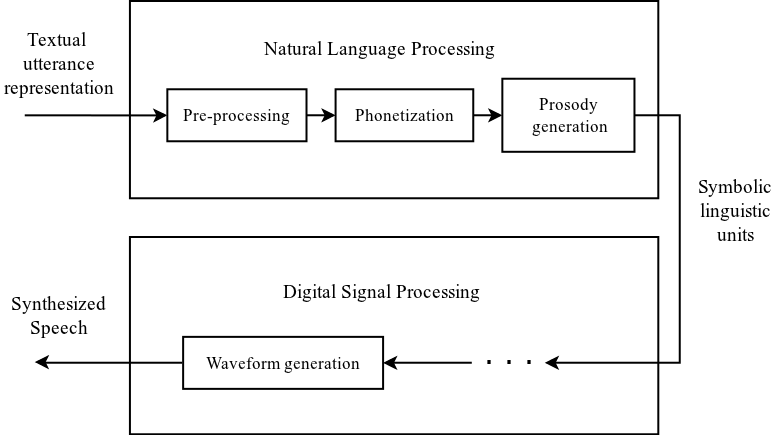
\includegraphics[width=0.5\textwidth]{figures/tts_system.png}
    \caption{Text-to-speech model \cite{speect}}
    \label{fig:tts}
\end{figure}

%%%%%%%%%%%%%%%%%%%%%%%%%%%%%%%%%%%%%%%%%%%%%%%%%%%%%%%%%%%%%%%%%%%%%%%%
\section{Probleemstelling}
%%%%%%%%%%%%%%%%%%%%%%%%%%%%%%%%%%%%%%%%%%%%%%%%%%%%%%%%%%%%%%%%%%%%%%%%

Vaak wordt gedacht dat het probleem van geschreven tekst vertalen naar spraak een probleem van 'omgekeerde spraakherkenning' is: huidige spraakherkenningssystemen worden als succesvol beschouwd als die opgenomen spraak kan vertalen naar de sequentie van woorden die zijn gezegd, dus men zou denken dat een TTS synthesizer begint bij de woorden in de tekst, die elk vertaalt naar een audio representatie, en de aparte resultaten aan elkaar hecht. Echter, het correct uitspreken van woorden is maar een onderdeel van spraak. Om een natuurlijke stem en een goede interpretatie van het gezegde te bewerkstelligen, moeten sommige woorden worden benadrukt en andere minder; een zin wordt op een betekenisvolle manier gefraseerd; er moet een gepaste contour van de $F_0$ (fundamentele) frequentie worden gekozen (de melodische contour in de stem), et cetera.

De moeilijkheid van de vertaalslag van tekst naar spraak, is het gebrek aan veel aspecten van informatie die van belang zijn voor spraak. Weliswaar representeert een zin alle woorden om de betekenis duidelijk te maken, maar het specificeert de frasering van een zin maar gedeeltelijk (door middel van bijvoorbeeld punctuatie), het specificeert niet de meer en minder benadrukte woorden en het geeft geen informatie over de intonatie of stemkwaliteit van een woord of frase.

TTS wordt vaak verdeeld in twee sub-problemen. Het eerste probleem adresseert de vertaling van tekst - een eigenlijk imperfecte representatie van taal zoals eerder aangegeven - in een linguïstieke vorm. Deze vorm bevat informatie over de fonemen die moeten worden geproduceerd, de duur en locaties van pauzeringen en de $F_0$ contour die moet worden gebruikt. Het tweede probleem adresseert de eigenlijke synthese van spraak. Het neemt de informatie uit het eerste probleem en vertaalt die naar een geluidsgolf.

Het eerste probleem, de tekst en linguïstieke analyse, wordt als volgt opgedeeld:
\begin{itemize}
    \item \textit{Tekst voorverwerking}: de detectie van het einde van de zin, tekst normalisatie (het volledig uitschrijven van nummers en afkortingen) en een grammaticale analyse, zoals het indelen van woorden in de bijbehorende, lexicale categorie (POS-tagging).
    \item \textit{Accentueren}: het aangeven van de nadruk die moet worden gelegd op bepaalde woorden.
    \item \textit{Uitspraak van woorden}: waarbij gelet wordt op de uitspraak van eigennamen, maar ook de desambiguatie van homoniemen \footnote{Een homoniem is een zelfstandig woord dat eenzelfde uitspraak heeft en tot eenzelfde woordsoort behoort, maar twee of meerdere geheel andere betekenissen heeft.}
    \item \textit{Fraseringen}: het fraseren van de zin door middel van intonatie.
    \item \textit{$F_0$ contour berekening}: waarbij een passende, melodische contour van de zin wordt berekend.
\end{itemize}

Het tweede probleem van spraak synthese wordt opgedeeld in twee delen:
\begin{itemize}
    \item de synthese van de spraak waveforms gegeven de gegenereerde, foneme delen in de eerste probleemstelling;
    \item de selectie en samenvoeging van zinsdelen gegeven de spraak waveforms.
\end{itemize}

%%%%%%%%%%%%%%%%%%%%%%%%%%%%%%%%%%%%%%%%%%%%%%%%%%%%%%%%%%%%%%%%%%%%%%%%
\section{Gesynthetiseerde stem}
%%%%%%%%%%%%%%%%%%%%%%%%%%%%%%%%%%%%%%%%%%%%%%%%%%%%%%%%%%%%%%%%%%%%%%%%

Text-to-speech synthese kent al een lange historie, beginnend bij Dudley's 'Voder' dat werd ontwikkeld bij Bell Laboratories en werd gedemonstreerd bij de World Fair in 1939 \cite{voder}. Een mens bestuurde de 10 bandpass filters van de 'Voder' om menselijke spraak te genereren. Pas vanaf de jaren '60 worden er systemen geïntroduceerd die automatisch spraak kunnen genereren op basis van linguïstieke representaties (zoals fonetische of tekstuele input). De twee belangrijkste technieken voor het synthetiseren van spraak waveforms zijn formantsynthese en concatinerende synthese (concatenative synthesis).

\subsection{Formantsynthese}
De eerste vorm van digitale spraaksynthese werd gerealiseerd met formantsynthese. Een formant is een smalle, piekende spectrale vorm die een oorsprong vindt in de resonantie van het menselijke spraakkanaal. Bij formantsynthese wordt gebruik gemaakt van additieve synthese en akoestieke modellering om spraak te genereren. Hierbij worden dus geen menselijke samples gebruikt.

\subsection{Concatenative synthesis}
Deze synthesetechniek synthetiseert geluid door middel van digitale, (korte) geluidssamples in een grote database slim te selecteren en samen te voegen (ook wel \textit{units} genoemd).

\subsubsection{Unit selection synthesis}
Een spraak synthesizer gebaseerd op concatenative synthesis gebruikt stukken natuurlijke spraak als bouwstenen om een arbritraire, nieuwe zin van spraak te reconstrueren \cite{nuance}. Een database van spraak \textit{units} is gemaakt met opnames van spraak. Door gebruik te maken van echte spraak worden een aantal karakteristieken van de stemacteur behouden. Een voordeel van \textit{Unit selection synthesis} is, dat wanneer er juiste \textit{units} worden gekozen, er een realistische stem met ook articulatie effecten ontstaat. Een ander voordeel is dat het een relatief eenvoudig systeem is, er hoeft weinig aandacht besteed te worden aan articulatie en synthese omdat er alleen gebruik wordt gemaakt van echte spraak \textit{units}.

In \textit{Unit selection synthesis} systemen wordt in een database gezocht naar foniemen die in dezelfde context als de \textit{target} foniemen voorkomen. Er wordt een \textit{penalty} voor het matchen van de gekozen foniem en de context gecaculeerd. Dit wordt gedaan door het verschil van de naburige foniemen in de \textit{target} en de naburige foniemen in de database te berekenen. De \textit{unit waveforms} van de \textit{target} worden daarna aan elkaar gezet (concatanation) door \textit{Pitch Synchronous Overlap and Add} (PSOLA) tussen aaneengesloten foniemen. Het algoritme past niet de prosodie aan, maar gebruikt dezelfde lengte, intonatie en articulatie van de foniem in de database. Het gebrek aan een goede, \textit{prosodic target} is een van de grootste tekortkomingen in dit systeem.

Om de ontwikkeling van een spraak \textit{unit} database te versnellen, zijn er automatische synthese \textit{unit} generation systemen ontwikkeld \cite{nakajima1994automatic}. Hierbij wordt de inventaris van spraak \textit{units} automatisch geannoteerd door middel van een al geannoteerde database (spraak waarvan de tekst al is getranscribeerd).


\subsubsection{Diphone synthesis}
ne popular unit is the diphone, which consists of the transition from the center of one phoneme to the center of the following one. This model helps to capture transitional information between phonemes. A complete set of diphones would number approximately 1600, since there

are approximately (40) possible combinations of phoneme pairs. Diphone speech synthesis thus requires only a mod erate amount of storage. One disadvantage of diphones is that they lead to a large number of concatenation points (one per phoneme), so that heavy reliance is placed upon an efficient Smoothing algorithm, preferably in combination with a diphone boundary optimization. Traditional diphone synthesizers, such as the TTS3000 of Lernout & Hauspie Speech and Language Products N.V., use only one candidate speech unit per diphone. Due to the limited prosodic vari ability, pitch and duration manipulation techniques are needed to synthesize speech messages. In addition, diphones synthesis does not always result in good output speech quality.



%%%%%%%%%%%%%%%%%%%%%%%%%%%%%%%%%%%%%%%%%%%%%%%%%%%%%%%%%%%%%%%%%%%%%%%%
\section{Hedendaagse technieken}
%%%%%%%%%%%%%%%%%%%%%%%%%%%%%%%%%%%%%%%%%%%%%%%%%%%%%%%%%%%%%%%%%%%%%%%%

\subsection{WaveNet}
WaveNet is een neuraal netwerk voor het genereren van audio waveforms \cite{45774}. Dit model is volledig probabilistisch en zelfvoorspellend, waarbij er een kansdistributie wordt berekend voor elk audio sample, geconditioneerd op alle vorige. Wanneer het wordt gebruikt in een tekst-to-speech toepassing, heeft het een state-of-the-art prestatie waarbij mensen het als significant beter en realistischer beoordelen dan de beste concatenative synthese systemen \footnote{\url{https://deepmind.com/blog/wavenet-generative-model-raw-audio}}. WaveNet kan ook worden gebruikt voor het herkennen van foniemen, voor bijvoorbeeld gebruik in concatenative synthesis.

WaveNet is ontwikkeld door DeepMind en ligt ten grondslag aan alle nieuwe text-to-speech systemen van Google die onder andere worden gebruikt in de Google Assistant \footnote{\url{https://cloud.google.com/text-to-speech/docs/wavenet}}.




\subsection{Tacotron}

\cite{Wang2017TacotronTE}
A text-to-speech synthesis system typically consists of multiple stages, such as a text analysis frontend, an acoustic model and an audio synthesis module. Building these components often requires extensive domain expertise and may contain brittle design choices. In this paper, we present Tacotron, an end-to-end generative text-to-speech model that synthesizes speech directly from characters. Given <text, audio> pairs, the model can be trained completely from scratch with random initialization. We present several key techniques to make the sequence-to-sequence framework perform well for this challenging task. Tacotron achieves a 3.82 subjective 5-scale mean opinion score on US English, outperforming a production parametric system in terms of naturalness. In addition, since Tacotron generates speech at the frame level, it's substantially faster than sample-level autoregressive methods. 


or machine translation (Wu et al., 2016),  TTS outputs are continuous,  and output sequences areusually much longer than those of the input. These attributes cause prediction errors to accumulatequickly.   In this paper,  we propose Tacotron,  an end-to-end generative TTS model based on thesequence-to-sequence (seq2seq) (Sutskever et al., 2014) with attention paradigm (Bahdanau et al.,2014).  Our model takes characters as input and outputs raw spectrogram, using several techniquesto improve the capability of a vanilla seq2seq model.   Given<text,  audio>pairs,  Tacotron canbe trained completely from scratch with random initialization.  It does not require phoneme-levelalignment, so it can easily scale to using large amounts of acoustic data with transcripts.  With asimple waveform synthesis technique, Tacotron produces a 3.82 mean opinion score (MOS) on anUS English eval set, outperforming a production parametric system in terms of naturalness1.


\subsection{Deep Voice}
\footnote{\url{https://r9y9.github.io/deepvoice3_pytorch/}}
We present Deep Voice 3, a fully-convolutional attention-based neural text-to-speech (TTS) system. Deep Voice 3 matches state-of-the-art neural speech synthesis systems in naturalness while training ten times faster. We scale Deep Voice 3 to data set sizes unprecedented for TTS, training on more than eight hundred hours of audio from over two thousand speakers. In addition, we identify common error modes of attention-based speech synthesis networks, demonstrate how to mitigate them, and compare several different waveform synthesis methods. We also describe how to scale inference to ten million queries per day on one single-GPU server. 


BAIDU \cite{Arik2017DeepVR}.
We present Deep Voice, a production-quality text-to-speech system constructed entirely from deep neural networks. Deep Voice lays the groundwork for truly end-to-end neural speech synthesis. The system comprises five major building blocks: a segmentation model for locating phoneme boundaries, a grapheme-to-phoneme conversion model, a phoneme duration prediction model, a fundamental frequency prediction model, and an audio synthesis model. For the segmentation model, we propose a novel way of performing phoneme boundary detection with deep neural networks using connectionist temporal classification (CTC) loss. For the audio synthesis model, we implement a variant of WaveNet that requires fewer parameters and trains faster than the original. By using a neural network for each component, our system is simpler and more flexible than traditional text-to-speech systems, where each component requires laborious feature engineering and extensive domain expertise. Finally, we show that inference with our system can be performed faster than real time and describe optimized WaveNet inference kernels on both CPU and GPU that achieve up to 400x speedups over existing implementations. 

\subsection{Mozilla Common Voice}

\subsection{Char2Wav}
\url{http://josesotelo.com/speechsynthesis/}

\subsection{Parrotron}
\cite{biadsy2019parrotron}
We describe Parrotron, an end-to-end-trained speech-to-speech conversion model that maps an input spectrogram directly to another spectrogram, without utilizing any intermediate discrete representation. The network is composed of an encoder, spectrogram and phoneme decoders, followed by a vocoder to synthesize a time-domain waveform. We demonstrate that this model can be trained to normalize speech from any speaker regardless of accent, prosody, and background noise, into the voice of a single canonical target speaker with a fixed accent and consistent articulation and prosody. We further show that this normalization model can be adapted to normalize highly atypical speech from a deaf speaker, resulting in significant improvements in intelligibility and naturalness, measured via a speech recognizer and listening tests. Finally, demonstrating the utility of this model on other speech tasks, we show that the same model architecture can be trained to perform a speech separation task 



\subsection{Tacotron 2}
\cite{Shen2018NaturalTS}
Natural TTS Synthesis by Conditioning WaveNet on Mel Spectrogram Predictions
This paper describes Tacotron 2, a neural network architecture for speech synthesis directly from text. The system is composed of a recurrent sequence-to-sequence feature prediction network that maps character embeddings to mel-scale spectrograms, followed by a modified WaveNet model acting as a vocoder to synthesize timedomain waveforms from those spectrograms. Our model achieves a mean opinion score (MOS) of 4.53 comparable to a MOS of 4.58 for professionally recorded speech. To validate our design choices, we present ablation studies of key components of our system and evaluate the impact of using mel spectrograms as the input to WaveNet instead of linguistic, duration, and F0 features. We further demonstrate that using a compact acoustic intermediate representation enables significant simplification of the WaveNet architecture. 

\footnote{\url{https://rayhane-mamah.github.io/Tacotron-2_audio_samples/}}

\subsubsection{Prosody embedding}
 In this work, we propose "global style tokens" (GSTs), a bank of embeddings that are jointly trained within Tacotron, a state-of-the-art end-to-end speech synthesis system. The embeddings are trained with no explicit labels, yet learn to model a large range of acoustic expressiveness. GSTs lead to a rich set of significant results. The soft interpretable "labels" they generate can be used to control synthesis in novel ways, such as varying speed and speaking style - independently of the text content. They can also be used for style transfer, replicating the speaking style of a single audio clip across an entire long-form text corpus. When trained on noisy, unlabeled found data, GSTs learn to factorize noise and speaker identity, providing a path towards highly scalable but robust speech synthesis. 

SAMPLES:
\url{https://ai.googleblog.com/2018/03/expressive-speech-synthesis-with.html}
\begin{figure}[]
    \centering
    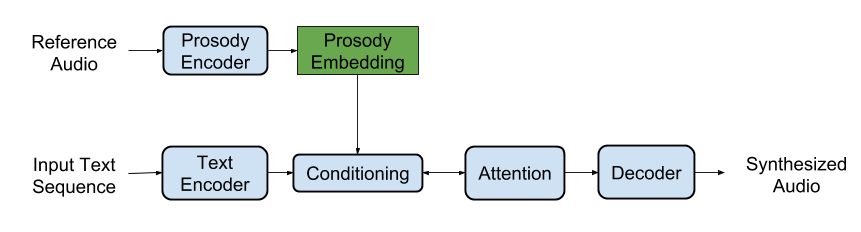
\includegraphics[width=0.75\textwidth]{figures/tacotron_prosody.png}
    \caption{Towards End-to-End Prosody Transfer for Expressive Speech Synthesis with Tacotron \cite{skerry2018towards}}
    \label{fig:tts}
\end{figure}

\subsection{WaveGlow}
\footnote{\url{https://nv-adlr.github.io/WaveGlow}}

%%%%%%%%%%%%%%%%%%%%%%%%%%%%%%%%%%%%%%%%%%%%%%%%%%%%%%%%%%%%%%%%%%%%%%%%

%%%%%%%%%%%%%%%%%%%%%%%%%%%%%%%%%%%%%%%%%%%%%%%%%%%%%%%%%%%%%%%%%%%%%%%%
\subsection{Sample Efficient Adaptive Text-to-Speech}

There is growing interest in developing neural TTS models that can be trained end-to-end withoutthe need for hand-crafted representations.  In this study we focus on extending the autoregressiveWaveNet model (van den Oord et al., 2016; 2017) to the few-shot learning setting to adapt to speakersthat were not presented at training time. Other recent neural TTS models include Tacotron 2 (Skerry-Ryan et al., 2018) (building on (Wang et al., 2017)) which uses WaveNet as a vocoder to invertmel-spectrograms generated by an attentive sequence-to-sequence model. DeepVoice 2 (Gibianskyet al., 2017) (building on (Arık et al., 2017)) introduced a multi-speaker variation of Tacotron thatlearns a low-dimensional embedding for each speaker, which was further extended in DeepVoice 3(Ping et al., 2018) to a 2,400 multi-speaker scenario. Unlike WaveNet and DeepVoice, the Char2Wav(Sotelo et al., 2017) and VoiceLoop (Taigman et al., 2018) models produce World Vocoder Features(Morise et al., 2016) instead of generating raw audio signals.Although many of these systems have produced high-quality samples for speakers present in thetraining set, generalizing to new speakers given only a few seconds of audio remains a challenge.There have been several concurrent works to address this few-shot learning problem. The VoiceLoopmodel introduced a novel memory-based architecture that was extended by Nachmani et al. (2018)to few-shot voice style adaptation,  by introducing an auxiliary fitting network that predicts theembedding of a new speaker.  Jia et al. (2018) extended the Tacotron model for one-shot speakeradaptation by conditioning on a speaker embedding vector extracted from a pretrained speaker identitymodel of Wan et al. (2018). The most similar approached to our work was proposed by Arik et al.(2018) for the DeepVoice 3 model. They considered both predicting the embedding with an encodingnetwork and fitting the embedding based on a small amount of adaptation data, but the adaptationwas applied to a prediction model for mel-spectrograms with a fixed vocoder.

\cite{chen2018sample}
\footnote{\url{https://sample-efficient-adaptive-tts.github.io/demo/}}

%%%%%%%%%%%%%%%%%%%%%%%%%%%%%%%%%%%%%%%%%%%%%%%%%%%%%%%%%%%%%%%%%%%%%%%%
\section{Afweging en advies}
%%%%%%%%%%%%%%%%%%%%%%%%%%%%%%%%%%%%%%%%%%%%%%%%%%%%%%%%%%%%%%%%%%%%%%%%

Het aanpakken van een aantal facetten van Prosody.
\url{7700-transfer-learning-from-speaker-verification-to-multispeaker-text-to-speech-synthesis (1).pdf}
%%%%%%%%%%%%%%%%%%%%%%%%%%%%%%%%%%%%%%%%%%%%%%%%%%%%%%%%%%%%%%%%%%%%%%%%
\chapter{Ontwikkelpotentie}
%%%%%%%%%%%%%%%%%%%%%%%%%%%%%%%%%%%%%%%%%%%%%%%%%%%%%%%%%%%%%%%%%%%%%%%%

\begin{center}
  \begin{minipage}{0.5\textwidth}
    \begin{small}
    \end{small}
  \end{minipage}
  \vspace{0.5cm}
\end{center}

%%%%%%%%%%%%%%%%%%%%%%%%%%%%%%%%%%%%%%%%%%%%%%%%%%%%%%%%%%%%%%%%%%%%%%%%
\section{Inleiding}
%%%%%%%%%%%%%%%%%%%%%%%%%%%%%%%%%%%%%%%%%%%%%%%%%%%%%%%%%%%%%%%%%%%%%%%%

Voor de in hoofdstuk 2.4 uitgelichte techieken is er veel data nodig om een realistisch gesynthetiseerde stem met menselijk en persoonlijk karakter te realiseren. In dit hoofdstuk wordt de beschikbaarheid van Nederlandse datasets onderzocht en toegelicht. Ook wordt er een schatting gemaakt over de benodigde kwantiteit en kwaliteit van de data om deze stem te realiseren.


%%%%%%%%%%%%%%%%%%%%%%%%%%%%%%%%%%%%%%%%%%%%%%%%%%%%%%%%%%%%%%%%%%%%%%%%
\section{Beschikbare Nederlandse datasets}
%%%%%%%%%%%%%%%%%%%%%%%%%%%%%%%%%%%%%%%%%%%%%%%%%%%%%%%%%%%%%%%%%%%%%%%%

\subsection{Corpus Gesproken Nederlands (CGN)}
Het Corpus Gesproken Nederlands is door het Instituut voor de Nederlandse Taal in 2014 ontwikkeld \footnote{\url{https://ivdnt.org/downloads/taalmaterialen/tstc-corpus-gesproken-nederlands}}. Deze dataset bevat 900 uur aan Nederlandse spraak, afkomstig van Vlamingen en Nederlanders. Dit maakt de dataset een \textit{multi-speaker} dataset, waarvan de uitdagingen al zijn uitgelijnd in het vorige hoofdstuk. Alle spraakfragmenten, in totaal 12.780, zijn getranscribeerd met orthografische en fonetische transcripties. Ook zijn ze syntaacticsh en met POS-tags (woordsoort informatie) geannoteerd. Het lexicon van deze dataset beslaat ongeveer 9 miljoen woorden. Deze dataset is ontworpen voor het testen van spraakherkennings software. In tabel \ref{tab:cgn} worden zijn alle spraakcategorieën onderverdeeld. Het gebruik van deze dataset is gratis, zowel voor niet-commercieel als commercieel gebruik, alhoewel er een licentie moet worden ondertekend voor het gebruik ervan.

Hoewel er veel goed geannoteerde, Nederlandse spraakdata aanwezig is in deze dataset, heeft deze een zeer heterogene samenstelling waarbij audiokwaliteit, stemkwaliteit, meerdere stemmen, de aanwezigheid van het Vlaams en context een belemmering vormen. Om deze reden is deze dataset niet geschikt om te worden gebruikt voor de eerder genoemde neurale netwerken. Wel is het geschikt als dataset voor een Nederlands speech-to-text systeem.

\begin{table}[]
    \centering
    \scalebox{0.75}{
        \begin{tabular}{l||c|c|c}
            Component & Totaal a. woorden & VL & NL \\
             Spontane conversaties ('face-to-face') & 2.626.172 & 878.383 & 1.747.789 \\
             Interviews met leraren Nederlands & 565.433 & 315.554 & 249.879 \\
             Telefoondialogen opgenomen m.b.v. telefooncentrale & 1.208.633 & 465.096 & 743.537 \\
             Telefoondialogen opgenomen m.b.v. minidiscrecorder & 853.371 & 343.167 & 510.204 \\
             Zakelijke onderhandelingen & 136.461 & 0 &  136.461 \\
             Interviews en discussies uitgezonden op radio en televisie & 790.269 & 250.708 & 539.561 \\
             Discussies, debatten, vergaderingen (m.n. politieke) & 360.328 & 138.819 & 221.509 \\
             Lessen & 405.409 & 105.436 & 299.973 \\
             Spontane commentaren (o.a. sport) uitgezonden op radio en televisie  & 208.399 & 78.022 & 130.377 \\
             Actualiteitenrubrieken en reportages uitgezonden op radio en televisie & 186.072 & 95.206 & 90.866 \\
             Nieuwsbulletins uitgezonden op radio en televisie & 368.153 & 82.855 & 285.298 \\
             Beschouwingen en commentaren uitgezonden op radio en televisie & 145.553 & 65.386 & 80.167 \\
             Missen, lezingen, plechtige toespraken & 18.075 & 12.510 & 5.565 \\
             Colleges, voordrachten, lezingen & 140.901 & 79.067 & 61.834  \\
             Voorgelezen teksten & 903.043 & 351.419 & 551.624  \\
             \textbf{Totaal} & \textbf{8.916.272} & \textbf{3.261.628} & \textbf{5.654.644}
        \end{tabular}
    }
    \caption{Corpus Gesproken Nederlands 	spraakcategorieën}
    \label{tab:cgn}
\end{table}

\subsection{LibriVox}
LibriVox is een website dat audioboeken, in het publieke domein aanbiedt. De boeken zijn ingesproken door vrijwilligers op het platform en zijn, hoewel niet altijd volledig professioneel opgenomen, van adequate kwaliteit om datasets van te maken. LibriVox heeft op het moment van schrijven 287 boeken in het Nederlands beschikbaar gesteld \footnote{\url{https://librivox.org/search?primary_key=19&search_category=language&search_page=1&search_form=get_results}}. Zoals eerder besproken, geniet het samenstellen van een homogene dataset met maximaal 1 stemacteur en veel uren spraakdata de voorkeur. Er zijn een aantal vrijwilligers die meerdere boeken hebben ingesproken, waaronder \textit{Marcel Coenders} met een catalogus van 112 voorgelezen boeken \footnote{\url{https://librivox.org/reader/2450?primary_key=2450&search_category=reader&search_page=1&search_form=get_results}}. In theorie is deze hoeveelheid spraakdata genoeg om een overtuigende stem te verkrijgen door middel van hedendaagse technieken (WaveNet, Tacotron 2).

LibriVox biedt alleen de audio opnames van de boeken aan. Een orthografische transcriptie opgelijnd aan de tekst wordt dus niet aangeboden, deze zal moeten worden samengesteld door middel van speech-to-text software en handmatig werk.

Een nadeel dat wordt genoemd in het gebruik van audioboeken als dataset, is dat de stemacteur vaak op geacteerde wijze de teksten voorleest. Dit heeft zeer mogelijk een impact op de gesynthetiseerde stem, waardoor voor commerciële implementaties gekozen wordt een volledig eigen dataset te maken met neutraal gesproken en gecureerde zinnen.

%%%%%%%%%%%%%%%%%%%%%%%%%%%%%%%%%%%%%%%%%%%%%%%%%%%%%%%%%%%%%%%%%%%%%%%%
\section{Oplijnen orthografische transcriptie}
%%%%%%%%%%%%%%%%%%%%%%%%%%%%%%%%%%%%%%%%%%%%%%%%%%%%%%%%%%%%%%%%%%%%%%%%
Voor deep learning text-to-speech technieken moet de dataset in een vorm worden gezet, zodat het netwerk de latente translatie kan maken tussen tekst en spraak. Doorgaans wordt spraakdata in fragmenten geknipt, waarbij elk audio fragment een apart bestand is en een zin bevat. Naast alle bestanden met audio fragmenten, wordt er ook een lijst bijgehouden van de orthografische transcriptie van de spraak per bestand. Deze lijst bestaat uit de kolommen zoals weergegeven in Tabel \ref{tab:orthografische_file}.

Voor het automatisch oplijnen en genereren van transcripties uit een spraakdata bestand, bevat het bestand ook tijdcodes van de start en eindpositie van de transcriptie in de spraakdata. Deze methode heet \textit{forced alignment}, waarbij audio en tekst met elkaar worden gesynchroniseerd. Een veelgebruikte, open-source software voor deze taak is \texttt{aeneas} \footnote{\url{https://github.com/readbeyond/aeneas}}. Hierbij wordt een bestand gegenereerd zoals aangegeven in Figuur \ref{fig:aenas}. 

\begin{table}[]
    \centering
    \scalebox{0.7}{
        \begin{tabular}{c|c|c}
            bestands naam & orthografische transcriptie & genormaliseerde, orthografische transcriptie \\
            librivox\_1.wav & Dhr. Koenders bestelde 46 tomaten bij de groenteboer. & De heer Koenders bestelde zes en veertig tomaten bij de groenteboer.
        \end{tabular}
    }
    \caption{Kolommen van een orthografisch transcriptie bestand}
    \label{tab:orthografische_file}
\end{table}

\begin{figure}
    \centering
    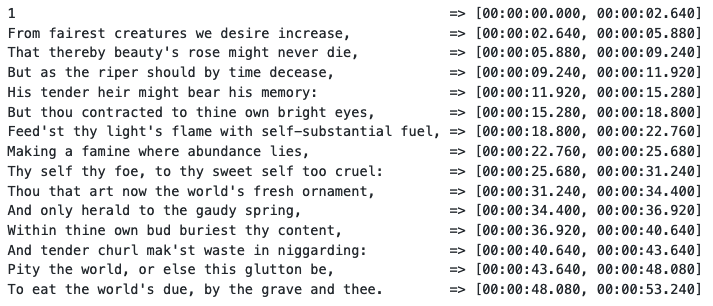
\includegraphics[width=0.75\textwidth]{figures/transcription.png}
    \caption{Voorbeeld bestand van een automatische, orthografische transcriptie met tijdcodes}
    \label{fig:aenas}
\end{figure}


\subsection{LJSpeech}
Hoewel dit een Engelse dataset betreft, wordt deze toch toegelicht door de unieke, homogene samenstelling en segmentatie ervan. LJSpeech is een spraak dataset in het publieke domein van 13.100 korte audio fragmenten van een spreker die passages leest van 7 verschillende non-fictie boeken. De audio fragmenten hebben een lengte van 1 tot 10 seconden, samenvattend bevat het ongeveer 24 uur aan spraak data. Alle audio fragmenten zijn orthografische getranscribeerd, zowel in de geschreven als gezegde (genormaliseerde) vorm. In de genormaliseerde vorm worden cijfers, de aanhef en andere afkortingen volledig uitgeschreven.

Elk audio fragment is een mono, 16-bit PCM WAV bestand met een sample rate van 22050 Hz. De LJSpeech dataset wordt vaak gebruikt in text-to-speech wedstrijden, workshops van conferenties en intern om modellen te testen. Het formaat en de omvang dient daarom als een streven voor het samenstellen van een Nederlandse variant. Ook kan deze dataset worden gebruikt als experiment om hypothesen op te toetsen en, met op het oog het budget, een ontwikkelrichting te maken voor een Nederlands gesynthetiseerde stem.

\begin{table}[H]
    \centering
    \begin{tabular}{c|c}
    Totaal a. fragmenten & 13,100 \\
    Totaal a. woorden & 225,715 \\
    Totaal a. karakters & 1,308,674 \\
    Totale lengte & 23:55:17 \\
    Gemiddelde lengte audio fragment & 6.57 sec \\
    Minimale lengte audio fragment & 1.11 sec \\
    Maximale lengte audio fragment & 10.10 sec \\
    Gemiddeld a. woorden per audio fragment & 17.23 \\
    Unieke woorden & 13,821 \\
    \end{tabular}
    \caption{LJSpeech dataset statistieken}
    \label{tab:ljspeech}
\end{table}


% LJ001-0002|in being comparatively modern.|in being comparatively modern.
% LJ001-0003|For although the Chinese took impressions from wood blocks engraved in relief for centuries before the woodcutters of the Netherlands, by a similar process|For although the Chinese took impressions from wood blocks engraved in relief for centuries before the woodcutters of the Netherlands, by a similar process
% LJ001-0004|produced the block books, which were the immediate predecessors of the true printed book,|produced the block books, which were the immediate predecessors of the true printed book,
% LJ001-0005|the invention of movable metal letters in the middle of the fifteenth century may justly be considered as the invention of the art of printing.|the invention of movable metal letters in the middle of the fifteenth century may justly be considered as the invention of the art of printing.
% LJ001-0006|And it is worth mention in passing that, as an example of fine typography,|And it is worth mention in passing that, as an example of fine typography,


\subsection{M-AILABS Speech Dataset}
M-AILABS heeft recentelijk een van de grootste, homogene spraakdatasets in het publieke domein uitgegeven
\footnote{\url{https://www.caito.de/2019/01/the-m-ailabs-speech-dataset/}}. De dataset bevat data van LibriVox en Project Gutenberg, met ongeveer duizend uur aan audio en tekst in totaal. Ook zijn de orthografische transcripties opgelijnd met de audio, wat deze dataset uniek in zijn soort maakt voor veel verschillende talen en stemkarakters. Het audioformaat is mono en 16.000 Hz. Het formaat is consistent met de LJSpeech dataset beschreven in de vorige sectie. De M-AILABS heeft veel verschillende talen, maar bevat geen Nederlandse spraakdata. Deze dataset is daarom niet geschikt voor het ontwikkelen van een Nederlandse stem, maar kan gebruikt worden om mee te experimenteren en een idee te krijgen van de benodigde grootte van de data voor een adequaat resultaat in een getraind neuraal netwerk.

%%%%%%%%%%%%%%%%%%%%%%%%%%%%%%%%%%%%%%%%%%%%%%%%%%%%%%%%%%%%%%%%%%%%%%%%
\section{Kwalitatieve en kwantitatieve analyse van spraakdata}
%%%%%%%%%%%%%%%%%%%%%%%%%%%%%%%%%%%%%%%%%%%%%%%%%%%%%%%%%%%%%%%%%%%%%%%%

Voor het Nederlands zijn er geen transcriptiebestanden aanwezig bij spraakdata van 1 spreker met meer dan of gelijk aan 24 uur aan spraakdata. Dit bemoeilijkt het samenstellen van een adequate dataset voor een text-to-speech systeem gebruikmakend van deep learning modellen. Naast dat de kwantiteit van spraakdata aangeboden door LibriVox voldoende is, is de kwaliteit ook geschikt voor het creëren van een realistisch, Nederlands sprekende gesynthetiseerde stem. De opnames zullen wel moeten worden opgelijnd door middel van automatische spraakherkkeningssoftware en handmatig werk.

Voor het creëren van een realistische, Nederlands sprekende stem wordt uitgegaan van minimaal 24 uur aan spraakdata van 1 spreker. Ook kan er voor worden gekozen een, wel homogene, \textit{multi-speaker} dataset te maken, alhoewel er significant meer data nodig is om een neuraal netwerk te laten generaliseren op de data. Het creëren van een zodanig netwerk is nodig, ook wanneer technieken als Prosody Embeddings of die geïntroduceerd in \textit{Sample Efficient Adaptive Text-to-Speech} gebruikt gaan worden. Er bestaan hedendaags geen vrij beschikbare, state-of-the-art getrainde (`pre-trained') modellen voor het Nederlands die kunnen worden gebruikt om Transfer Learning of eerdergenoemde technieken te gebruiken. Deze getrainde modellen worden nu vaak in het Engels of Chinees aangeboden, en zijn ook niet optimaal getraind zodat de commerciële positie van de opdrachtgever van het onderzoek niet in gevaar komt (zoals de gepubliceerde modellen van Deepmind, Google en Baidu).

Wanneer er een \textit{baseline} stem is getraind en geïmplementeerd, kan met een aantal minuten spraakdata van een andere spreker al snel een nieuwe stem worden ontwikkeld. Dit is beschreven in \textit{Sample Efficient Adaptive Text-to-Speech}, maar is nog niet getest in andere talen dan het Engels. Mogelijk kan ook een stem worden ontwikkeld met een ander, eigen karakter en een (licht) accent nadat deze \textit{baseline} stem is ontwikkeld.

%%%%%%%%%%%%%%%%%%%%%%%%%%%%%%%%%%%%%%%%%%%%%%%%%%%%%%%%%%%%%%%%%%%%%%%%
\section{Handmatig werk}
%%%%%%%%%%%%%%%%%%%%%%%%%%%%%%%%%%%%%%%%%%%%%%%%%%%%%%%%%%%%%%%%%%%%%%%%
Voor het creëren van een correct, orthografisch transcriptie bestand is handmatig werk noodzakelijk. Automatische speech-to-text systemen hebben, zeker voor het Nederlands, een Word Error Rate (WER) die te hoog kan liggen om een adequate transcriptie te verkrijgen. Daarom is het hebben of ontwikkelen van annotatiesoftware noodzakelijk om dit op een gestroomlijnde wijze te bewerkstelligen. Vaak wordt dit werk uitbesteed aan bijvoorbeeld instanties als Amazon Mechanical Turk, die gespecialiseerd is in het inzetten van menselijk denken in het maken van AI datasets. Een open-source annotatie implementatie specifiek voor \textit{forced alignment}, is \texttt{finetuneas} \footnote{\url{https://github.com/ozdefir/finetuneas}}. Het is ontworpen om de orthografische transcriptie output van \texttt{aeneas} eenvoudig te manipuleren en te corrigeren\ref{fig:finetuneas}. Doorgaans kost het correct annoteren van een uur spraakdata 8 á 10 uur werk\label{benodigd_werk}. Voor een dataset van minimaal 24 uur, komt dit neer op 192 uur. Door gebruik te maken van een automatisch speech-to-text systeem kan dit proces worden versneld. Wel geldt, dat de audio van goede kwaliteit moet zijn en de speech-to-text software de gesproken taal ondersteund. Met name geldt dit voor dialect: huidige speech-to-text software hebben een hoge Word Error Rate wanneer het dialect moet transcriberen. Een Nederlandse stem ontwikkelen met dialect benodigd dus significant meer handmatig werk om een correcte orthografische transcriptie te vervaardigen waar een neuraal netwerk getraind mee kan worden.

\begin{figure}[H]
    \centering
    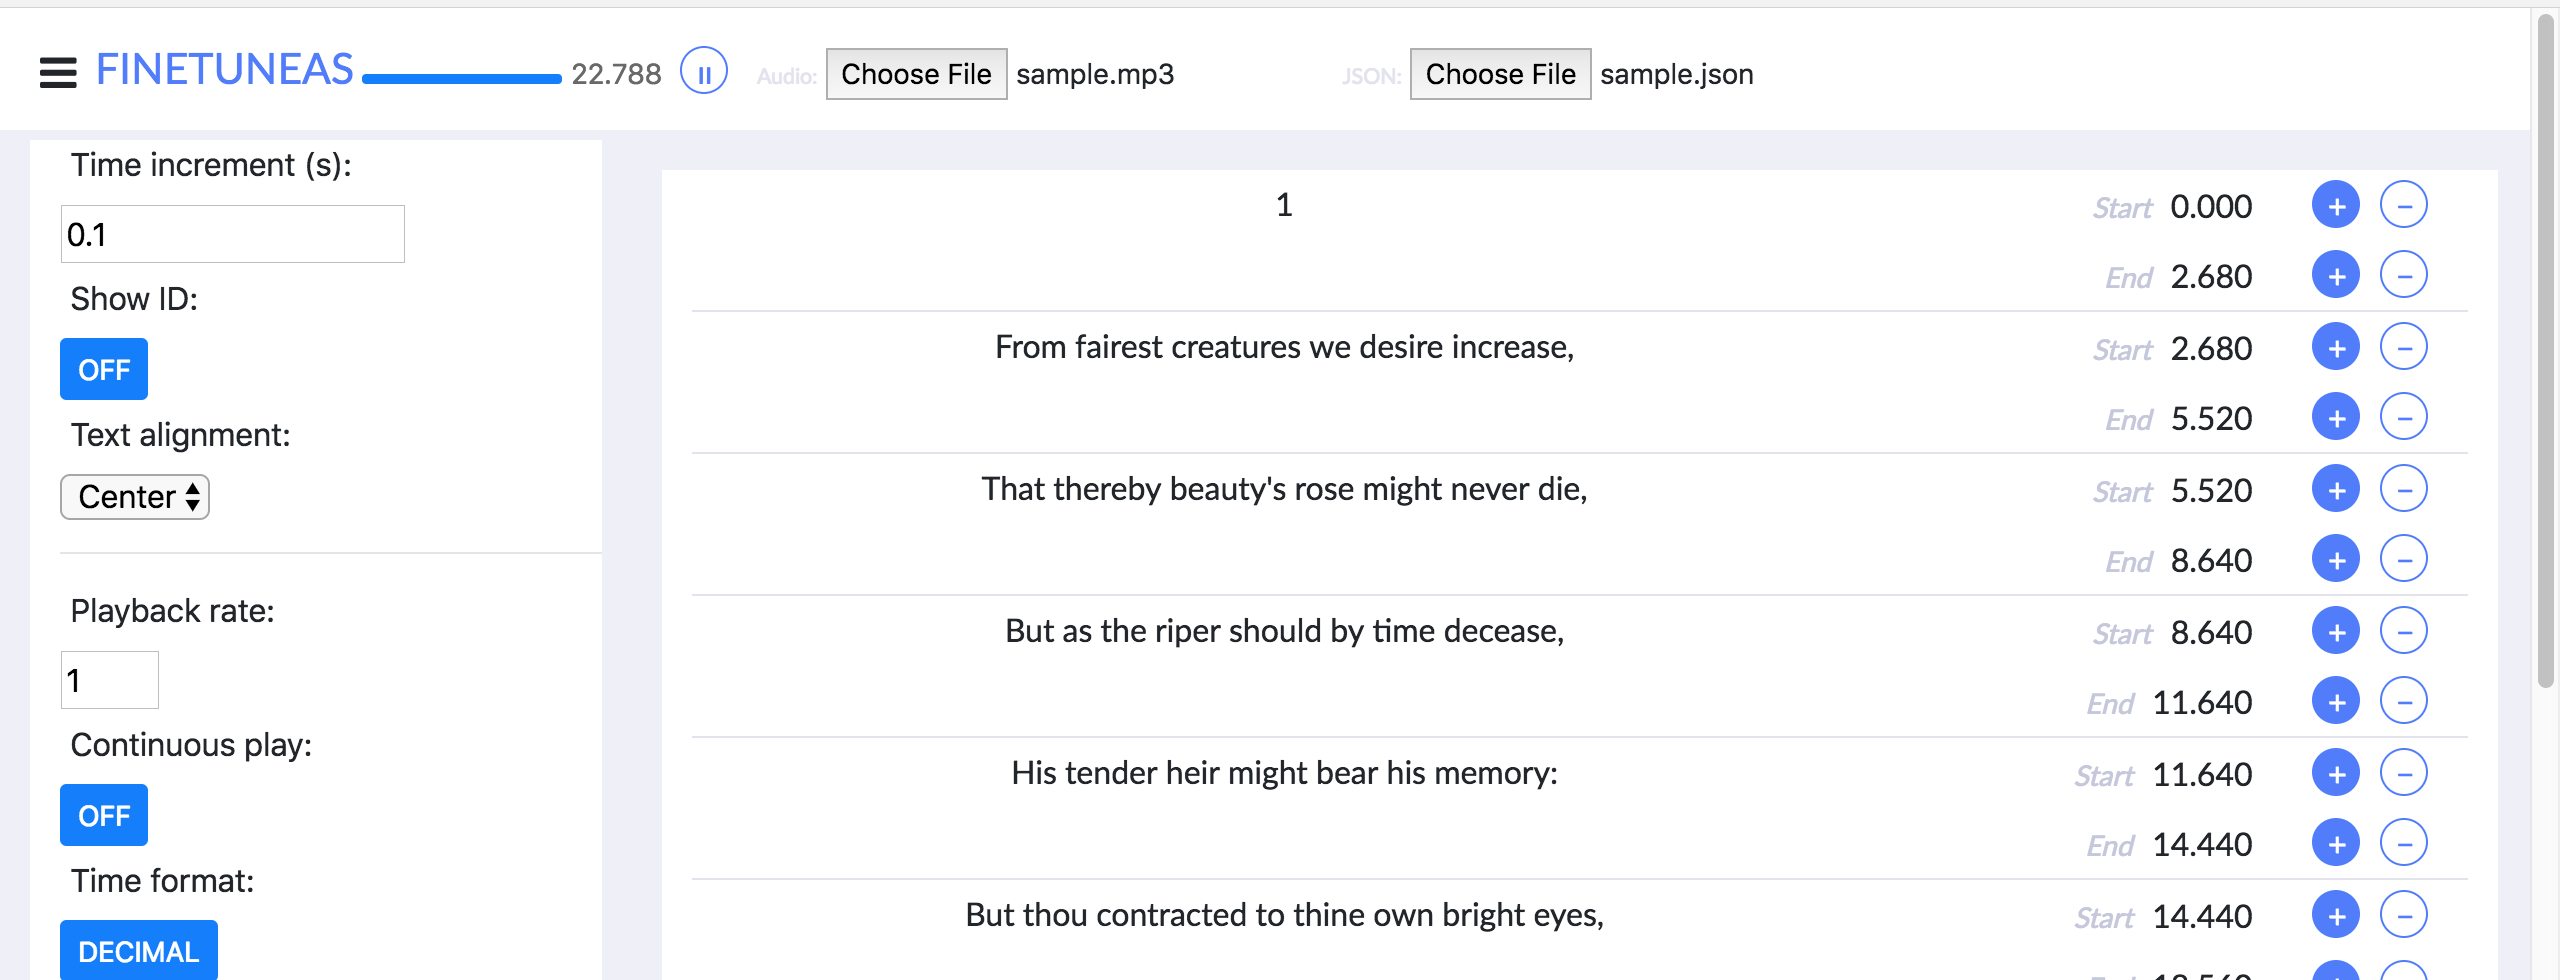
\includegraphics[width=\textwidth]{figures/finetuneas.png}
    \caption{Web interface van \texttt{finetuneas}}
    \label{fig:finetuneas}
\end{figure}

%%%%%%%%%%%%%%%%%%%%%%%%%%%%%%%%%%%%%%%%%%%%%%%%%%%%%%%%%%%%%%%%%%%%%%%%

\section{Conclusies ontwikkelpotentie}
%%%%%%%%%%%%%%%%%%%%%%%%%%%%%%%%%%%%%%%%%%%%%%%%%%%%%%%%%%%%%%%%%%%%%%%%

Het CGN is een te heterogene dataset om adequaat een neuraal netwerk mee te trainen zoals WaveNet of Tacotron. Een netwerk als Deep Voice 3 werkt beter op \textit{multi-speaker} datasets, dus die combinatie kan een uitkomst bieden, maar is minder gegarandeerd. LibriVox kan dienen als een eerste opzet naar het ontwikkelen van een homogene, Nederlandstalige dataset om een model als WaveNet of Tacotron 2 te trainen, waarbij de voorkeur uitgaat naar Tacotron 2 omdat een correcte implementatie al vrij beschikbaar is. Het gebruik van automatische speech-to-text voor Standaardnederlands met \texttt{aeneas} wordt aangeraden voor de \textit{forced alignments}, waarbij de audio met de spraak wordt gesynchroniseerd. Handmatige aanpassingen kunnen daarna worden gedaan met \texttt{finetuneas}.

Wanneer er een \textit{baseline} stem is getraind met een homogene dataset, kunnen de gegeven, optimale \textit{weights} van het getrainde netwerk gebruikt worden om, met een aantal minuten spraakdata van een andere spreker, een stemvariant te ontwikkelen met \textit{Sample Efficient Adaptive Text-to-Speech}, hoewel dit nog niet is getest in andere talen dan het Engels. Dit biedt ook de mogelijkheid tot het ontwikkelen van een stemvariant met een ander, eigen karakter en een (licht) accent, gegeven dat deze \textit{baseline} stem volledig is ontwikkeld.
%%%%%%%%%%%%%%%%%%%%%%%%%%%%%%%%%%%%%%%%%%%%%%%%%%%%%%%%%%%%%%%%%%%%%%%%
\chapter{Ontwikkelrichting}
%%%%%%%%%%%%%%%%%%%%%%%%%%%%%%%%%%%%%%%%%%%%%%%%%%%%%%%%%%%%%%%%%%%%%%%%

\begin{center}
  \begin{minipage}{0.5\textwidth}
    \begin{small}
      In which the reasons for creating this package are laid bare for the
      whole world to see and we encounter some usage guidelines.
    \end{small}
  \end{minipage}
  \vspace{0.5cm}
\end{center}

%%%%%%%%%%%%%%%%%%%%%%%%%%%%%%%%%%%%%%%%%%%%%%%%%%%%%%%%%%%%%%%%%%%%%%%%
\section{Inleiding}
%%%%%%%%%%%%%%%%%%%%%%%%%%%%%%%%%%%%%%%%%%%%%%%%%%%%%%%%%%%%%%%%%%%%%%%%
In dit hoofdstuk wordt een aantal varianten van een ontwikkelrichting geschetst, rekening houdend met de opgaven waar Prolody B.V. voor staat. De varianten komen voort gegeven de technieken uitgelijnd in hoofdstuk 2 en de beschikbare data in hoofdstuk 3.

%%%%%%%%%%%%%%%%%%%%%%%%%%%%%%%%%%%%%%%%%%%%%%%%%%%%%%%%%%%%%%%%%%%%%%%%
\section{Variant A}
%%%%%%%%%%%%%%%%%%%%%%%%%%%%%%%%%%%%%%%%%%%%%%%%%%%%%%%%%%%%%%%%%%%%%%%%
De eerste variant wordt als volgt gedefinieerd: het ontwikkelen van een Standaardnederlands sprekende stem, zonder dialec, door het professioneel opnemen van een stemacteur. Dit wordt gedaan met ongeveer 24 uur spraak data, waarbij automatische speech-to-text herkenning wordt uitgevoerd met \texttt{aeneas}, waarna handmatige aanpassingen binnen het \texttt{finetuneas} systeem worden gedaan.

Het dan gegenereerde orthografische transcriptie bestand wordt met de audio samples gebruikt om Tacotron 2 te trainen. De parameters van het netwerk worden daarna handmatig versteld, totdat er een acceptabel, eerste resultaat wordt behaald. Als vervolgstap kunnen andere stemmen, met eventueel dialect, worden gegenereerd door middel van de technieken uitgelijnd in \textit{Sample Efficient Adaptive Text-to-Speech}. Omdat er relatief weinig spraakdata nodig is om een stemvariant te maken, is dit een reële optie om te onderzoeken of op een eenvoudige wijze een stem met een ander karakter kan worden ontwikkeld. Ook kan na het trainen van een Standaardnederlandse stem worden gekeken naar Prosody Embeddings om de stem te verbeteren voor het signaalpad tussen robot en mens.

%%%%%%%%%%%%%%%%%%%%%%%%%%%%%%%%%%%%%%%%%%%%%%%%%%%%%%%%%%%%%%%%%%%%%%%%
\section{Variant B}
%%%%%%%%%%%%%%%%%%%%%%%%%%%%%%%%%%%%%%%%%%%%%%%%%%%%%%%%%%%%%%%%%%%%%%%%
De tweede variant wordt als volgt gedefinieerd: het ontwikkelen van een Nederlands sprekende stem, met dialect, door het professioneel opnemen van een stemacteur. Dit wordt wederom gedaan met ongeveer 24 uur spraak data, waarbij automatische speech-to-text herkenning wordt uitgevoerd met \texttt{aeneas}, waarna handmatige aanpassingen binnen het \texttt{finetuneas} systeem worden gedaan. Echter, de Word Error Rate van text-to-speech systemen is erg hoog vergeleken met het Standaardnederlands. Deze variant zal dus significant meer handmatig werk benodigen. Het dan gegenereerde orthografische transcriptie bestand wordt met audio samples gebruikt om Tacotron 2 te trainen. De parameters van het netwerk worden daarna handmatig versteld, totdat er een acceptabel, eerste resultaat wordt behaald.

Deze variant geeft hoogstwaarschijnlijk het meest realistische resultaat, maar is zeer mogelijk beperkt in adaptief gebruik in het creëren van andere stemvarianten. Ook is deze variant het meest arbeidsintensief.

%%%%%%%%%%%%%%%%%%%%%%%%%%%%%%%%%%%%%%%%%%%%%%%%%%%%%%%%%%%%%%%%%%%%%%%%
\section{Variant C}
%%%%%%%%%%%%%%%%%%%%%%%%%%%%%%%%%%%%%%%%%%%%%%%%%%%%%%%%%%%%%%%%%%%%%%%%
De derde variant wordt als volgt gedefinieerd: het ontwikkelen van een Nederlands sprekende stem, gebruik makende van een bestaande, Nederlandse spraak dataset zoals de audioboeken in LibriVox. Hoewel de data in het publieke domein ligt, moet worden onderzocht of de data volledig vrij te gebruiken is. Weer is minimaal 24 uur aan spraakdata benodigd, dat gedeeltelijk automatisch door speech-to-text herkenning met \texttt{aeneas} wordt omgezet in een orthografische transcriptie. De transcriptie kan daarna handmatige worden verbeterd binnen het \texttt{finetuneas}. Het gegenereerde en verbeterde orthografische transcriptie bestand wordt met de audio samples gebruikt om Tacotron 2 te trainen. De parameters van het netwerk worden daarna aangepast totdat er een acceptabel, eerste resultaat wordt behaald.

De kwaliteit van de audio van het resultaat is afhankelijk van de kwaliteit van de spraakdataset. Er zal dus moeten worden gelet op de uitvoering van de gekozen LibriVox dataset. Ook moet de dataset homogeen zijn, waarbij de voorkeur uit gaat naar maximaal 1 stemacteur.

%%%%%%%%%%%%%%%%%%%%%%%%%%%%%%%%%%%%%%%%%%%%%%%%%%%%%%%%%%%%%%%%%%%%%%%%
\section{Variant D}
%%%%%%%%%%%%%%%%%%%%%%%%%%%%%%%%%%%%%%%%%%%%%%%%%%%%%%%%%%%%%%%%%%%%%%%%
De vierde variant betreft vooral een experimenteel alternatief op de vorige vier, waarbij gebruik wordt gemaakt van een bestaande, Engelse spraak dataset zoals \textit{LJSpeech}. Met deze dataset kan dan worden geëxperimenteerd met de best werkende deep learning modellen voor spraakdata en het, nadat het netwerk is getraind, creëren van stemvarianten door middel van de technieken uitgelijnd in \textit{Sample Efficient Adaptive Text-to-Speech}. Met deze variant kan Prolody B.V. eerst onderzoeken welke stappen binnen een ontwikkelrichting moeten worden genomen om tot een gewenst resultaat te komen, zonder dat er veel kosten en arbeidsuren worden gemaakt.

Een nadeel van deze variant, is dat er geen Nederlands sprekende stem wordt ontwikkeld, noch een deep learning model voor Nederlanse text-to-speech wordt getraind die kan worden ingezet om andere stemvarianten te maken zoals de gewenste variatie in dialect en accent.
% Fries / Drenths Speech to Text
%%%%%%%%%%%%%%%%%%%%%%%%%%%%%%%%%%%%%%%%%%%%%%%%%%%%%%%%%%%%%%%%%%%%%%%%
\chapter{Financiële haalbaarheid}
%%%%%%%%%%%%%%%%%%%%%%%%%%%%%%%%%%%%%%%%%%%%%%%%%%%%%%%%%%%%%%%%%%%%%%%%

\begin{center}
  \begin{minipage}{0.5\textwidth}
    \begin{small}
    \end{small}
  \end{minipage}
  \vspace{0.5cm}
\end{center}

%%%%%%%%%%%%%%%%%%%%%%%%%%%%%%%%%%%%%%%%%%%%%%%%%%%%%%%%%%%%%%%%%%%%%%%%
\section{Inleiding}
%%%%%%%%%%%%%%%%%%%%%%%%%%%%%%%%%%%%%%%%%%%%%%%%%%%%%%%%%%%%%%%%%%%%%%%%

Het uitschrijven van één uur geluid kost ongeveer 8 á 10 uur werk en is dus erg arbeidsintensief en dus erg duur. Automatische spraakherkenning (ASR = Automatic Speech Recognition) is snel en erg goedkoop, maar helaas maken de spraakherkenningsprogramma’s nog wel veel fouten. In de toekomst zal dit zeker beter gaan, maar op dit moment worden ongeveer 20% van de woorden nog niet goed herkend.%%%%%%%%%%%%%%%%%%%%%%%%%%%%%%%%%%%%%%%%%%%%%%%%%%%%%%%%%%%%%%%%%%%%%%%%

%%%%%%%%%%%%%%%%%%%%%%%%%%%%%%%%%%%%%%%%%%%%%%%%%%%%%%%%%%%%%%%%%%%%%%%%
\section{Financiële parameters}
%%%%%%%%%%%%%%%%%%%%%%%%%%%%%%%%%%%%%%%%%%%%%%%%%%%%%%%%%%%%%%%%%%%%%%%%
De prijzen die zijn uitgelijnd in deze paragraaf zijn opgevraagd in april 2019.


%%%%%%%%%%%%%%%%%%%%%%%%%%%%%%%%%%%%%%%%%%%%%%%%%%%%%%%%%%%%%%%%%%%%%%%%
\section{Hardware}
%%%%%%%%%%%%%%%%%%%%%%%%%%%%%%%%%%%%%%%%%%%%%%%%%%%%%%%%%%%%%%%%%%%%%%%%

Tacotron 2 gebruikt circa 11GB GPU memory met een \texttt{batch\_size} van van 32. Het originele paper gebruikt een \texttt{batch\_size} van 64, waarmee state-of-the-art resultaten werden behaald. Hoe hoger de \texttt{batch\_size}, des te meer samples een neuraal netwerk `ziet'. Hiermee kunnen netwerken beter getraind worden, dan dat er lagere \texttt{batch\_size} worden gekozen.  Een GPU met minimaal 11 GB aan RAM wordt dus aanbevolen.

Er zijn drie kenmerken waar gelet op moet worden bij de aanschaf van een GPU voor het gebruik in deep learning:
\begin{enumerate}
    \item Geheugen (RAM): De mogelijkheid om veel data te processen. Veel hedendaagse deep learning modellen hebben grote datasets en een diepe netwerk structuur, waardoor veel geheugen nodig is bij het trainen van het netwerk. Voor het verwerken van beeld en audio wordt een hoger RAM aangeraden.
    \item Processing kracht: Dit geeft aan hoe snel de GPU data kan verwerken. Dit wordt vaak berekend aan de kloksnelheid en het aantal CUDA cores van de GPU. 
\end{enumerate}

Een snelle GPU is belangrijk voor het snel ontwikkelen van de architectuur van het model en het aanpassen van de parameters. Het kan vaak uren tot dagen duren voordat een netwerk convergeert naar een resultaat. Wanneer er dan fouten zijn gemaakt, kost het veel tijd om het netwerk opnieuw op te starten en te trainen. In een test is Tacotron 2 \footnote{\url{https://github.com/NVIDIA/tacotron2}} voor een aantal epochs getraind op een NVIDIA GTX 1080 Ti. (Een epoch is een gehele iteratie door de gehele dataset). Een iteratie over een batch kostte ongeveer 3 seconden, waardoor een epoch ongeveer 15 minuten bedroeg. In totaal worden 500 epochs voorgeschreven, wat neerkomt op ongeveer 5 dagen in totaal om Tacotron 2 te trainen op de LJSpeech dataset op een NVIDA GTX 1080 Ti.

De nieuwe 'Volta' generatie van NVIDIA GPU's hebben een een Tensor Core unit. Deze zijn significant sneller en worden hedendaags veel gebruikt bij het trainen van diepe netwerken. In tabel \ref{tab:gpus} worden de kosten uitgelicht van drie verschillende modellen, waarmee een onderscheid wordt gemaakt in de GTX, Kepler en Volta generaties.

\begin{table}[H]
    \centering
    \begin{tabular}{c|c|c|c|c}
        Hardware & CUDA cores & RAM & TFLOPS &  Kosten \\
        NVIDIA GTX 1080 Ti & 3584 & 11 GB & 1.079 & \$700 \\
        NVIDIA Tesla K80 & 4992 &  24 GB & 1.87+ & \$1,700 \\
        NVIDA Tesla V100 & 5120 & 16 / 32 GB & 7 tot 7.8 & \$6,099 \\
    \end{tabular}
    \caption{Caption}
    \label{tab:gpus}
\end{table}

\subsection{AWS}
De onderstaande prijslijst is afkomstig van Amazon Web Services, dat instanties van cloud computers aanbiedt aan particulieren. De P-serie biedt GPU cloud computing instanties aan met NVIDIA Kepler en Volta GPU's.

\begin{table}[H]
    \centering
    \begin{tabular}{c|c|c|c|c|c}
        Model & GPU & vCPU & RAM & GPU RAM & Kosten (per maand) \\
        p2.xlarge & 1 $\times$ NVIDIA Tesla K80 & 4 & 61 & 12 & \$448.22  \\
        p2.8xlarge & 8 $\times$ NVIDIA Tesla V100 & 32 & 488 & 96 & \$3,587.22  \\
        p3.2xlarge & 1 $\times$ NVIDIA Tesla V100 & 8 & 61 & 16 & \$1,524.24 \\
        p3.8xlarge & 4 $\times$ NVIDIA Tesla V100 & 32 & 244 & 64 & \$6,098.42  \\
    \end{tabular}
    \caption{Caption}
    \label{tab:my_label}
\end{table}




%%%%%%%%%%%%%%%%%%%%%%%%%%%%%%%%%%%%%%%%%%%%%%%%%%%%%%%%%%%%%%%%%%%%%%%%
\section{Resultaten variant A}
%%%%%%%%%%%%%%%%%%%%%%%%%%%%%%%%%%%%%%%%%%%%%%%%%%%%%%%%%%%%%%%%%%%%%%%%

%%%%%%%%%%%%%%%%%%%%%%%%%%%%%%%%%%%%%%%%%%%%%%%%%%%%%%%%%%%%%%%%%%%%%%%%
\section{Resultaten variant B}
%%%%%%%%%%%%%%%%%%%%%%%%%%%%%%%%%%%%%%%%%%%%%%%%%%%%%%%%%%%%%%%%%%%%%%%%

%%%%%%%%%%%%%%%%%%%%%%%%%%%%%%%%%%%%%%%%%%%%%%%%%%%%%%%%%%%%%%%%%%%%%%%%
\section{Resultaten variant C}
%%%%%%%%%%%%%%%%%%%%%%%%%%%%%%%%%%%%%%%%%%%%%%%%%%%%%%%%%%%%%%%%%%%%%%%%

%%%%%%%%%%%%%%%%%%%%%%%%%%%%%%%%%%%%%%%%%%%%%%%%%%%%%%%%%%%%%%%%%%%%%%%%
\section{Resultaten variant D}
%%%%%%%%%%%%%%%%%%%%%%%%%%%%%%%%%%%%%%%%%%%%%%%%%%%%%%%%%%%%%%%%%%%%%%%%


%%%%%%%%%%%%%%%%%%%%%%%%%%%%%%%%%%%%%%%%%%%%%%%%%%%%%%%%%%%%%%%%%%%%%%%%
\section{Conclusie}
%%%%%%%%%%%%%%%%%%%%%%%%%%%%%%%%%%%%%%%%%%%%%%%%%%%%%%%%%%%%%%%%%%%%%%%%

% Voorbeeld van prosodie annotatie
%%%%%%%%%%%%%%%%%%%%%%%%%%%%%%%%%%%%%%%%%%%%%%%%%%%%%%%%%%%%%%%%%%%%%%%%
\chapter{Conclusies en aanbevelingen}
%%%%%%%%%%%%%%%%%%%%%%%%%%%%%%%%%%%%%%%%%%%%%%%%%%%%%%%%%%%%%%%%%%%%%%%%

\begin{center}
  \begin{minipage}{0.5\textwidth}
    \begin{small}
    \end{small}
  \end{minipage}
  \vspace{0.5cm}
\end{center}

\noindent This package contains a minimal, modern template for writing your
thesis. While originally meant to be used for a Ph.\,D.\ thesis, you can
equally well use it for your honour thesis, bachelor thesis, and so
on---some adjustments may be necessary, though.

%%%%%%%%%%%%%%%%%%%%%%%%%%%%%%%%%%%%%%%%%%%%%%%%%%%%%%%%%%%%%%%%%%%%%%%%
\section{Conclusies}

%%%%%%%%%%%%%%%%%%%%%%%%%%%%%%%%%%%%%%%%%%%%%%%%%%%%%%%%%%%%%%%%%%%%%%%%

\section{Aanbevelingen}

%%%%%%%%%%%%%%%%%%%%%%%%%%%%%%%%%%%%%%%%%%%%%%%%%%%%%%%%%%%%%%%%%%%%%%%%


% This ensures that the subsequent sections are being included as root
% items in the bookmark structure of your PDF reader.
% Soundscape Annotation Tool

% Ground up vs. Style Transfer

\bookmarksetup{startatroot}
\backmatter

  \begingroup
    \let\clearpage\relax
    \glsaddall
    \printglossary[type=\acronymtype]
    \newpage
    \printglossary
  \endgroup

\printindex
\printbibliography
\label{section:bibliography}
\end{document}
